% %This is a very basic article template.
% %There is just one section and two subsections.
\documentclass{article}

\usepackage[ colorlinks=true, urlcolor=blue, linkcolor=green ]{hyperref}
\usepackage[title]{appendix}

\usepackage{graphicx}

\begin{document}

\title{Group Proposal}

\author{Dr. Levi L\'ucio}
 
\maketitle

\abstract{We propose the creation of new nachwuchs-Kompetezfeld at fortiss in
the area of Domain Specific Languages (DSLs).}

\section{Name}

Intelligent Domain-Specific Systems (IDS2)

\section{Mission} 

\textbf{Increasingly build better DSLs to tackle industrial problems by:
1) applying them to implement and support technology transfer projects at
fortiss, and 2) evaluating their practical impact.}
 
\section{Need}

Computer languages are pervasive in software and systems engineering, to the
point that software engineers become unaware that the choice of the language set
to use plays a major role in projects' success. 

The IDS2 group aims at making DSLs a primary theme of concern at fortiss. Many
projects implemented at fortiss have a strong language development component. As
as such the group will be flexible in the range of projects it will acquire and
develop. The cross-section between IDS2 and other groups at fortiss is wide:
learning to design better languages will empower ourselves and other scientists
at fortiss to better transfer their results into industry. Additionally, DSLs
are a powerful tool to add robustness to fortiss' contributions in software
engineering.

Better technology transfer implies economical benefits for our industrial
partners and ultimately more business for fortiss itself.

\section{Business Model}

Industry is constantly on the lookout for automation that can provide an edge
regarding their competitors. This is particularly true in Bavaria, where large
automotive, aerospace and software companies exist and compete in a globalised
market.

While it is expected and understood that new techniques and tools will provide
such competitive edge, even large companies with dedicated research departments
cannot perform their own research in-house due to time or expertise constraints.

The IDS2 group will work hand-in-hand with industry to provide solutions to
software development problems that may be solved using domain-specific
languages. This is a proven business model: for example itemis AG or PROTOS GmbH
are currently using it with success. Both companies are expert in
their own modelling frameworks (MPS and eTrice respectively) and provide domain-specific
solutions based on those tools. Their areas of expertise of their clients range
from automotive, to aerospace, health, heavy machinery or manufacturers of power
tools.

Given fortiss' technology transfer mission, IDS2 does not intend to specialize
in one specific technological platform but rather to build expertise around the
the construction and evaluation of Domain-Specific Languages. In particular, we
intend on leveraging and experimenting with machine learning as well as with
practical formal methods in order to consistently provide innovative and
cutting-edge solutions.

When implementing projects with the industry we will follow a formula that has
proven successful in the past: for each project we intend on building a
prototype focused on solving one specific problem, delivering the solution in a
fashion such that the advantages of the research idea are clearly transmitted to
the industry. In practice, this means that our focus will not be on building an
encompassing framework where all solutions may be plugged in, but rather to
impress our clients with clean and clear-cut solutions to well-specified
problems. Technology will be used opportunistically and towards specific goals.

We strongly believe that such an approach will be impactful, as it is well
understood that the industry does not use prototypes built by fortiss directly
-- they rather re-implement the research idea for their proprietary toolchains when
the research is deemed to be useful. Equally important, such an approach will
allow us to build a range of impressive prototypes that will not only serve as a
presentation portfolio for the group, but will also allow us to attract more
business for fortiss.

\section{Scientific Contribution}

% The history of software engineering is one of inventing increasing levels of
% abstraction as a means to cope with the increasing complexity of software
% systems. High level languages such as C, Pascal or FORTRAN introduced
% programmers to structured code, C++, Java or C\# added the notion of
% \emph{object} as a means to encapsulate code. UML, together with design
% patterns, gave software developers principles of architecture and design.

% Software modelling is a broad term that proposes many different approaches to the different stages
% of software development (requirements, design, coding and
% verification/validation), making use of formal, semi-formal and informal
% languages. Based on the principles of software modelling, several tools such as
% Enterprise Architect or MATLAB Simulink have had significant impact in the
% industry.

% One of the currently most promising approaches to again raise the level of
% abstraction at which software is built are Domain-Specific Languages (DSLs).
% DSLs propose encapsulating the entities of the domain on which computations are
% to be performed through languages that encapsulate and manipulate the concepts
% of that same domain. Here, the Turing machine stops being the absolute reference
% -- rather, it becomes important to adjust the computational power to the task
% at hand. DSLs thus concentrate on providing adequate abstractions to describe
% computations for specific domains. They abstract from the machine-
% architecture- and mathematical-oriented properties of Turing-machine inspired
% languages and favor abstractions closer to the human understanding of the domain
% of interest.
% 
% During the past decade a number of DSL workbenches saw the light of day. The
% Eclipse Modelling Framework (EMF) had significant impact in the academia and
% became one of the most popular frameworks for DSL construction. More recently,
% the MPS workbench from Jetbrains has delivered a powerful DSL construction
% workbench with professional support and possibilities to design attractive GUIs
% that provide a very interesting complement to the notion of domain specificity.
% Professional DSL workbenches such as MetaEdit+ have repeatedly made strong cases
% for the industrial adoption of DSLs and have gathered a niche market in the
% domain.

% During the past few years, DSLs have attracted considerable interest from the
% industry. The paradigm speaks directly to engineers who wish to build their
% systems ground-up and making as much use as possible of domain knowledge that is
% typically hard-earned. In this context, clients often regard DSLs as key-in-hand
% solutions. They encompass simplified means to express domain-specific
% computations while abstracting from accidental complexity linked to the software or the hardware
% running underneath.
% 
% Companies such as itemis, PROTOS or MetaCase have successfully developed
% business models around DSLs. They leverage their knowledge of modelling and DSL workbenches to
% deliver to customers key-in-hand software solutions. Such solutions have been
% developed for disparate domains such as the automotive, avionics, power tools or
% health, biology, among many others, and help either software developers or final
% users in achieving their tasks.
 
% Despite these successes, the potential and real impact of DSLs in industry is
% still ill understood. A recent compelling report from Tolvanen and
% Kelly~\cite{Tolvanen016} states that while their company specialized in
% DSLs, MetaCase, can affirm with certainty that the gains in productivity of
% their clients range from 500\% to 1000\%. In the same article, they claim
% academic research in the domain thus not been able to validate this in general.
% They speculate this is due on the one hand to the quality of their tool
% MetaEdit+ and their industrial experience, and on the other hand to the poor
% quality of the academic tools for supporting DSL construction.

Anecdotally, at the PAINS workshop at MODELS 2018, an interesting discussion
raged between a high-profile DSL proponent and a top-level BMW manager. While
the DSL proponent insisted that the (MPS-based) technology was ready and could
serve as a ``silver bullet'' of sorts, the BMW manager replied that the attempts of using
DSLs at his company where ``hit-and-miss'' and that even when DSLs did prove
successful, it was not understood why. A question from that same manager that
was particularly thought-provoking was: ``how do I build and abstraction and
know that it is a good one?''. A more general criticism to the DSL approach in
general was: ``quality standards are missing, how do I to judge or trust your
processes of building DSLs while making decisions that will benefit my company?''.

\paragraph{Summary}
From the condensed state of the art in the !!! ATTACHED DOCUMENT !!! , we can
identify the following tends:

\begin{itemize}
  \item For almost two decades professional DSL workbench builders have
  consistently reported case studies of application of DSLs to industrial
  problems, some of those case studies being highly successful.
  The same DSL builders do nonetheless mention that obtaining the data for
  validating the DSL after shipment is difficult~\cite{Tolvanen018}.
  \item During that same period academia as struggled to provide evidence that
  the promises of DSLs in terms of increased productivity hold. Only recently,
  partly due to the arrival of mature DSL workbenches produced by professional
  software, is actual quantification of properties of DSLs such as e.g.
  usability becoming possible. Experimental validation of DSLs based on
  established theory is still under-explored~\cite{Mernik17}.
  \item The DSL workbenches developed by academia are, thus far, insufficient to
  scientifically validate the premises of the DSL-based software development.
  This is on the one hand due to the poor quality of the tooling
  produced by academia~\cite{TolvanenKelly2016}, and on the other hand to very
  low access to real industrial use cases. Most of the surveys we describe above use as study
  material other academic papers, leading to starvation of information on real
  DSL commercial usage.
  \item With the notable exceptions of the work of Tolvanen and Kelly and
  Völter mentioned above in this section, the bridges between the academia and
  industry in the DSL domain are brittle. 
\end{itemize}

\begin{figure}[!h]
\centering 
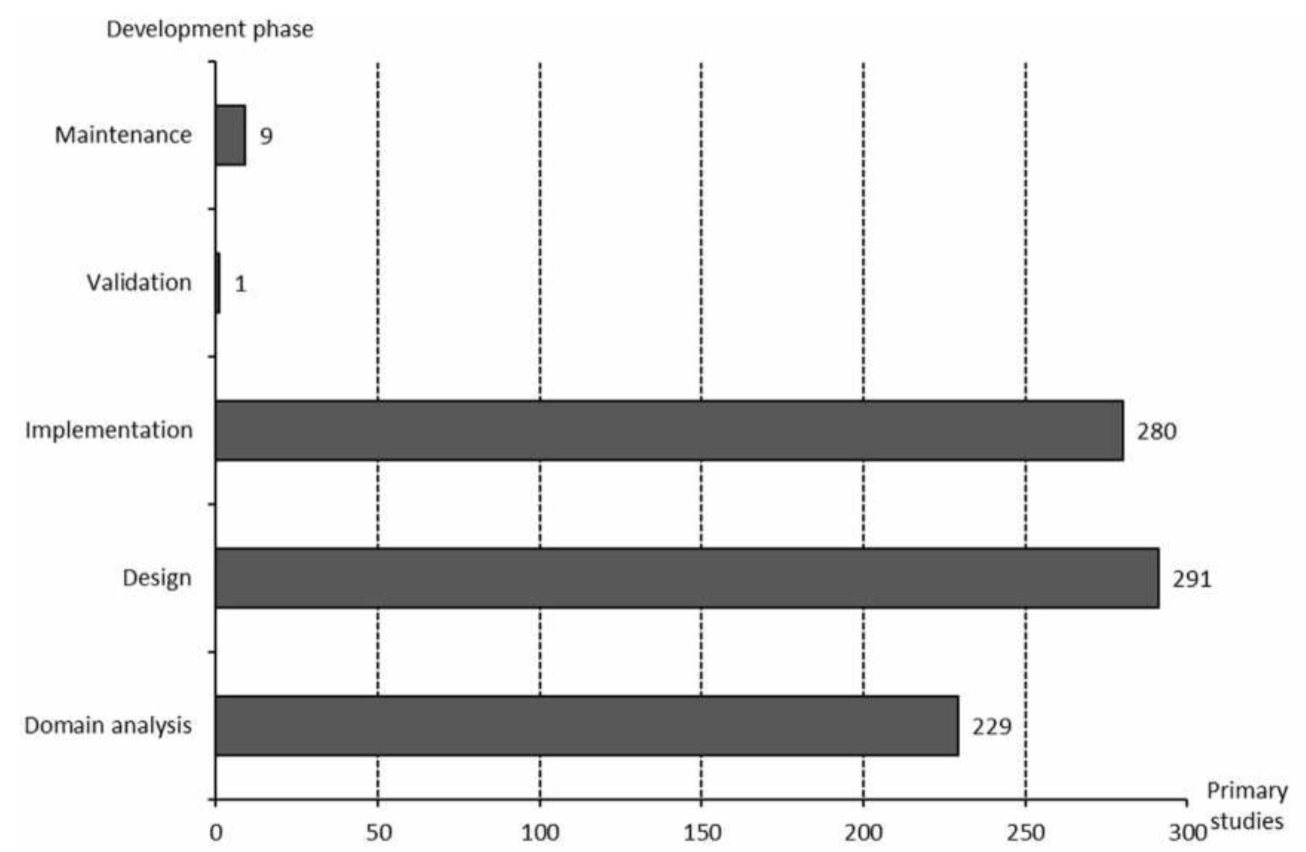
\includegraphics[width=1\textwidth]{./figures/DSL_design_phases}
\caption{Distribution of 810 scientific contributions according to the phases
of DSL construction they cover (extracted from~\cite{Mernik17})}
\label{fig:DSL_design_phases}
\end{figure}
!!! MAKE REF TO PIC !!!

IDS2 will be in a privileged position to find answers to the questions
above. The proposed main members of the group have considerable experience with
DSL workbenches, modelling and verification, both through their studies and their
professional accomplishments. Additionally, we rely on a national and
international academic and industrial network that is stable and currently
growing.

By developing DSLs for the industry as the main business model, we have and will
be exposed to the difficulties in the conception of DSLs, in their adoption and
evaluation in practice.\\

\textbf{Our main goal is to build a conceptual and systematic framework to build
DSLs and the right level of abstraction for the task at hand, as well as
evaluating their impact in the productivity of the industry and
discovering best practices.}\\

RQ1: What is the quality of an abstraction in a DSL?
RQ2: How do formal methods and machine learning help out?

Our mid-to-longterm goal is to inseminate the community with the practical
experiences and struggles of applying DSLs in practice, leading to the
theoretical establishment of the domain. fortiss is a very privileged context to
do this, as we have the kind of access to projects and partners that occurs very
seldom in academia. 

\section{Proposed Group Members}

\begin{itemize}
  \item Dr. Levi L\'ucio (group lead)
  \item Dr. Saad Bin Abid (topic leader for process modelling and machine
  learning)
  \item Sudeep Kanav (topic leader for formal methods in practice)
  \item Ananya Misra (HiWi)
  \item Vishal Mahajan (HiWi)
\end{itemize}

Dr. Saad Bin Abid and Sudeep Kanav have expressed keen interest on becoming part
of the IDS2 group. They are nonetheless members of MbSE and are
expected to work part-time for IDS2 where synergies exist. Depending on acquired
funds in 2019 and personal and group interests the percentage of time they work
for each group might be subjected to adjustments.

\section{Synergies with other groups at fortiss}

Domain-Specific Languages are a cross-cutting theme at fortiss. All
competence fields at fortiss deal with DSLs in one form or the
other, even or despite doing it unknowingly.

\begin{itemize}
\item The obvious synergy of IDS2 is with the MbSE group: MbSE has a
model-centric view on systems and software engineering and builds languages using model-driven
techniques. Its main current theme is design-space exploration and the modelling
of  embedded systems, but other themes such as requirements engineering, formal
methods or security are also being pursued. ID2S can be of great assistance to
MbSE by bringing systematic notions of language construction and evaluation to
the development table. A collaboration that is already ongoing is the
exploration of machine learning (in the context of the MAGNET project) to deliver support to users of AF3.
\item Common work is also ongoing with the AS group, in the form of the
FaktorBUILD project proposal. Some of the work of AS relies on probabilistic
programming to model situations where incomplete knowledge must be reliably used
to make decisions in real-time. Here, IDS2 may help in constructing DSLs at an
adequate level of abstraction such that the IDE provided to users of factor
graphs can leverage good abstractions, static analyses and formal methods to
increase the productivity of factor graph programmers.
\item The collaboration with the i4 group has been so far very successful,
having lead to the implementation (together with Vincent Aravantinos) of a tool
providing DSLs to express industrial capabilities. Such capabilities, or
skills, can be subsequently be matched to automatically automatically synthesize
controllers for industrial machines. Upcoming work for 2019 in the area will aim
at connecting the completed DSL-based tool to AutomationML and 4Diac in order
to connect the work with outside formats while providing simulation capabilities. 
\end{itemize}

\pagebreak

\begin{appendices}
\section{Context}

The proposal for the formation of this group stems from three years of work at
fortiss developing DSLs in the context of several projects. The three main
members of the foreseen group (Dr. Levi L\'ucio, Dr.
Saad Bin abid and Sudeep Kanaav) all have extensive experience working together
both for the IETS3 the CBMD and the MAGNET projects.

\subsection{Completed Projects}

\begin{itemize}
  \item IETS3
  \begin{itemize}
    \item Consortium: fortiss, itemis, ZF, Diehl aerospace
    \item Running time, funding and personnel: 2 years / ~300K Euro / 3 people
  \end{itemize}
\end{itemize}

\subsection{Running Projects}
\label{section:running_projects}

\begin{itemize}
  \item CBMD (as project leader)
  \begin{itemize}
    \item Consortium: fortiss, PROTOS, SQMi, University of Augsburg
    \item Running time, funding and personnel: 2 years / ~190K Euro / 2 people
  \end{itemize} 
  \item MAGIC (as project leader)
  \begin{itemize}
    \item Consortium: fortiss, University of Montréal
    \item Running time and funding: 2 years / ~10K Euro + ~40K Euro
    (Eigenforshungsgeld) / 3 people
  \end{itemize} 
  \item MAGNET (as project leader)
  \begin{itemize}
    \item Consortium: fortiss
    \item Running time, funding and personnel: 6 months / ~70K Euro / 8 people
    Eigenforshungsgeld
  \end{itemize}
  \item ARTEMIS (as project leader)
  \begin{itemize}
    \item Consortium: fortiss, Airbus
    \item Running time, funding and personnel: 6 months / 75KEuro / 2 people
    (Levi + HiWi)
  \end{itemize} 
  \item BaSys4.0 (as software developer for the ``industrial skills'' theme )
\end{itemize}

\subsection{Projects in the Acquisition Pipeline}
\label{section:projects_in_pipepline}

\begin{itemize}
  \item FaktorBUILD
    \begin{itemize}
    \item Consortium: fortiss, University of L\"ubeck, Siemens, LMU, ?
    \item Running time, funding and personnel: 3 years / ~400K Euro / 3 people
    (Levi + Dhiraj + HiWi)
  \end{itemize} 
  \item Follow-up for CBMD
    \begin{itemize}
    \item Consortium: fortiss, PROTOS, ?
  \end{itemize} 
  \item Follow-up for ARTEMIS
    \begin{itemize}
    \item Consortium: fortiss, Airbus
  \end{itemize} 
  \item H2020, project on ``agility in model-based software engineering''
    \begin{itemize}
    \item Consortium: fortiss, University of Antwerp, University Nova de Lisboa,
    TU Wien, Hasso-Platner Institut, Telecom-Paristech, Unit Bilisim
    Technologies
  \end{itemize} 
\end{itemize}

\section{Network}

Here I will describe the main currently active research and industrial
connections (others exist that may be reactivated at need):\\\\
\textbf{Inside fortiss:}

\begin{itemize}
  \item HCE (Yuanting Liu and team, project MAGNET)
  \item SD (Tahira Iqbal and Parisa Elahidoost, project MAGNET and requirements
  engineering)
  \item i4 (project MAGIC, networking with University of Montréal)
  \item AS (Dhiraj Gulati and Vincent Aravantinos, on BaSys and FactorBUILD)\\
\end{itemize}
\textbf{Academic}:

\begin{itemize}
  \item University of Montr\'eal, Canada (project MAGIC)
  \item University of Namur, Belgium (tutorial and paper on machine learning and
  formal verification)
  \item University of Antwerp, Belgium (proposal for H2020)
  \item LMU, Germany (with Prof. Dirk Beyer in the context of the FaktorBUILD
  proposal)
  \item University of L\"ubeck, Germany (with Prof. Philipp Rostalski in the
  context of the FactorGraph proposal)
  \item TU Wien (with Manuel Wimmer in the context of model transformations)\\
\end{itemize}
\textbf{Industrial:}

\begin{itemize}
  \item PROTOS (KMU) (in the context of the CBMD project)
  \item Rolls-Royce (in the context of the EARS-related work)
  \item Siemens (in the context of the FaktorBUILD proposal)
  \item Festo (in the context of the BaSys project)
  \item ABB (in the context of the BaSys project)
\end{itemize}

\section{Plan for the first year of activity}

In the first year of activity we intend on solidifying the group by building on
existing results and enlarging the scope of our national and international
network, both at the academic and industrial levels. In particular, we aim at
achieving the following goals:

\subsection{Research:}

\begin{itemize}
  \item Establish a set of criteria for the quality of DSLs in practice. In
  particular, we are interested in understanding which measurable criteria can
  be used to facilitate the adoption of DSLs in the industry.
  \item Evaluate the usage of machine learning in the context of requirements
  engineering and in general as a means to aid in the construction and operation
  of good and reliable DSLs.
  \item Establish an ongoing collaboration with Prof. Dirk Beyer from the LMU in
  Munich. Prof. Beyer is an expert in formal methods and is part of the
  consortium for the FaktorBUILD project. He is, in particular, very
  enthusiastic about applying his CPAchecker C model checker to examples coming
  from Airbus Defense in the context of the ARTEMIS project. Publishing with
  Prof. Beyer will also be pursued.
  \item Evaluate the prototype developed for the MAGNET project in the
  real-world scenario of tutorials of AF3. Calibrate the suggestions provided by
  the machine learning algorithm in function of such an evaluation.
  \item Write one or more articles on the results of the MAGNET project.
  \item Evaluate the usage of machine learning in the context of requirements
  engineering and in general as a means to aid in the construction and operation
  of good and reliable DSLs.
\item Establish a set of criteria for the quality of DSLs in practice. In
particular, I am interested in understanding which measurable criteria can be used to
facilitate the adoption of DSLs in the industry.
  \item Write one or more articles on the results of the skills (F\"ahigkeiten)
  work-package of the BaSys project.
 \item Continue research on the topic of Process-Aware model driven development
environments to be implemented in AF3. Complete the ongoing journal paper on
process-aware model-driven development environments.
 \item Help Sudeep Kanav in establishing his PhD research topic by publishing
 results on compositional model checking at top venues. Continue Sudeep's
 scientific training.
 \item Provide Tatiana Chuprina with the right tools such that she can finish
 her thesis proposal in the area of requirements engineering.
\end{itemize}

\subsection{Project acquisition:}

\begin{itemize}
  \item Build on our existing collaboration with Airbus defense by delivering
  excellent results for the ARTEMIS project and acquiring a second project in
  the context of model checking C code based on EARS requirements.
  \item Acquire one or more national and/or international projects. This work
  will be based on current acquisition efforts for a BMBF and an H2020 projects
  (as described in section~\ref{section:projects_in_pipepline}).
  \item Acquire a project on the continuation fn CBMD on the compositional
  verification of models of embedded software. This is well underway and desired
  by PROTOS GmbH (as described in sections~\ref{section:running_projects}
  and~\ref{section:projects_in_pipepline}).
  \item Acquire a project with an industrial partner (PROTOS is a promising
  option) on applying the results of MAGNET Eigenforshungs project in practice.
  \item Work in the direction of establishing a funded consortium with
  Professors Eugene Syriani and Michalis Famelis from the University of
  Montr\'eal. A collaboration with those researchers is already in place in the
  context of the MAGIC project (as described in~\ref{section:running_projects}) with the goal of acquiring a
  large Canadian-Germany partnership
  project\footnote{\url{http://www.nserc-crsng.gc.ca/International-Internationale/CanadaGermany_call-Appel_CanadaAllemagne_fra.asp}}.
\end{itemize}

\subsection{Technical:}

\begin{itemize}
  \item Build a prototype tool in MPS to generate LTL from EARS requirements and
  model-check C code written for those requirements. 
  \item Build a release-ready prototype of a recommender system for AutoFOCUS3
  that can be effectively used in tutorials on the tool given to industry or
  academia.
  \item Complete the development of the skill-matching and controller
  synthesis prototype for BaSys. The prototype will semi-automatically generate
  a controller for a robotic arm in 4Diac. A demonstrator of the complete chain
  from skill definition down to robot arm movement will be built based on
  virtual robotic arm simulator provided by Festo AG. 
  \item Integrate compositional model checking in the eTrice tool, such that it
  can be used in production by PROTOS.
\end{itemize}

\subsection{Organisation:}

\begin{itemize}
  \item Contribute to and aid in the delivery of tutorials for AF3.
  \item Contribute to the organization of MODELS 2019 in Munich.
  \item Conduct interviews leading to the the hiring of post-docs, PhD students,
  Msc students or HiWis.
\end{itemize}

\end{appendices}

\end{document}
 